\documentclass{report}

% Packages
\usepackage[T1]{fontenc}
\usepackage[utf8]{inputenc}
\usepackage[frenchb]{babel}
% \usepackage[english]{babel}
\usepackage[a4paper,width=170mm,top=18mm,bottom=22mm,includeheadfoot]{geometry}

\usepackage{titlesec}
\usepackage{graphicx}
\usepackage{listings}
\usepackage{color}
\usepackage{amsmath}
\usepackage{hyperref}

\definecolor{lightgray}{gray}{0.75}
\titleformat{\chapter}[hang]{\Huge\bfseries}{\thechapter\hspace{20pt}\textcolor{lightgray}{|}\hspace{20pt}}{0pt}{\Huge\bfseries}

\lstset{
    language=C,
    basicstyle=\small\sffamily,
    numbers=left,
    numberstyle=\tiny,
    frame=tb,
    tabsize=4,
    columns=fixed,
    showstringspaces=false,
    showtabs=false,
    keepspaces,
    showtabs=false,
    morekeywords={*, include, GET, POST, PUT, DELETE, let, u8, u16, u32, u64, use, pub, mut, trait, where, fn, self, Result, new, var, using, public, namespace, foreach},
    commentstyle={\color{gray}\textit},
    keywordstyle=\color{blue},
    stringstyle=\color{green}
}

\hypersetup{
    colorlinks=true,
    linkcolor=black,    % color of internal links (change box color with linkbordercolor)
    citecolor=black,    % color of links to bibliography
    filecolor=black,    % color of file links
    urlcolor=blue       % color of external links
}

% Document metadata
\title{
    \huge Données centralisées et intelligences interconnectées \\
    \LARGE Un Système pour les gouverner tous
}
\author{
    Valentin \textsc{Fries} \\ Master Architecture des Logiciels 
    \and
    Vincent \textsc{Milano} \\ Master Architecture des Logiciels
    \and
    Benjamin \textsc{Raynal} \\ Docteur en Vision par ordinateur \\ Maître de mémoire
}
%\date{} % Defaults to compilation date.
 
% Document
\begin{document}

\pagenumbering{gobble}
\maketitle

%\chapter*{Remerciements}
Cupidatat proident ullamco do eu reprehenderit veniam pariatur consectetur esse exercitation adipisicing enim duis. Nostrud voluptate dolore quis adipisicing esse. Minim aute sunt est fugiat proident veniam. Veniam enim consectetur laborum sit non.
\section*{Résumé}
\paragraph{} Qu'adviendrait-il si nos données personnelles étaient centralisées ?
\paragraph{} Si des IA interconnectées ou des systèmes de Machine Learning distribués parvenaient à les exploiter ?
\paragraph{} Smartphones, objets connectés, réseaux sociaux et démocratisation de la robotique : quels socles pour une société de contrôle ?

% Quels moyens nous sont donnés, aujourd'hui,
% pour parvenir à créer un système de contrôle
% omniscient ?

\newpage
\section*{Abstract}
Exercitation ad aliquip occaecat deserunt ipsum aliqua eiusmod incididunt. Ad excepteur mollit nostrud elit. Do qui sit sint elit ut ullamco proident incididunt eiusmod. Nisi labore ea et deserunt nulla cupidatat aute. Irure deserunt non qui eu nostrud nulla laboris nostrud irure. Amet minim officia sunt sunt do quis enim amet veniam.
 

\tableofcontents
\pagenumbering{arabic}

\chapter{Introduction}

\paragraph{} Nous vivons dans un monde complexe, aliénant, en perpétuel mouvement mais qui
nous incite à l'inaction. Réseaux sociaux, smartphones, objets connectés... Aujourd'hui, la
technologie a envahi notre quotidien d'une manière à la fois ostentatoire et subtile, outil
pervers satisfaisant au moindre de nos désirs.

\paragraph{} La question peut donc être posée sans rougir : disposons-nous, à l'heure
actuelle, des moyens nécessaires pour parvenir à la création d'un système de contrôle des
masses, d'un \emph{Système Omniscient} ?

\paragraph{} Prenez le temps d'y réfléchir. Toutes les briques sont déjà présentes autour
de vous : informations personnelles, centres d'intérêt, photos de toutes sortes, relations
et interactions sociales, messagerie instantanée et \emph{micro-blogging}, géolocalisation,
cursus scolaire et professionnel, recherches en ligne et historique des consultations,
informations bancaires, médicales, pièces d'identité... Êtes-vous réellement maître de vos
données ?

\paragraph{} Notre étude sera menée en trois parties, couplant chacune un sujet de réflexion
et d'analyse avec un prototype technique qui prendra de l'ampleur au fil de l'évolution de
notre pensée.

\paragraph{} Dans un premier temps, nous nous focaliserons sur les différents phénomènes
et modèles sociétaux ayant conduit à une intrication profonde de la technologie à notre
quotidien. Il sera question de mettre l'accent sur la récolte et l'aggrégation des données
\emph{"personnelles"} et sur les raisons qui peuvent motiver une telle collecte, pour ensuite
nous questionner sur les conséquences sur les comportements humains.

\paragraph{} Dans un second temps, notre étude portera sur les possibilités de mise en place
d'une telle solution, notamment à travers l'utilisation d'un réseau distribué. Hardware,
systèmes d'exploitation, contraintes techniques et environnementales... Quels sont les challenges
architecturaux d'une telle solution ? Nous verrons que l'Homme, à son échelle, facilite la 
construction de ces systèmes.

\paragraph{} Enfin nous chargerons-nous de doter notre prototype d'intelligence. Qu'est-ce que
l'Intelligence Artificielle ? Quelle est d'ores et déjà sa place dans nos systèmes actuels ?
Comment le Machine Learning permet-il aux innovations d'aujourd'hui de résoudre des problèmes
jusqu'alors inabordés ? Suite à l'implémentation de solutions algorithmiques complexes,
nous nous questionnerons alors sur l'éthique associée à ces sujets. Déterminisme,
eugénisme, améliorations de vie et sociales : il est important d'en questionner l'usage.

\paragraph{}  Qu'adviendrait-il si nos données personnelles étaient centralisées ? Si des IA interconnectées
ou des systèmes de Machine Learning distribués parvenaient à les exploiter ? Smartphones,
objets connectés, réseaux sociaux et démocratisation de la robotique : quels socles pour une
société de contrôle ?
\chapter{Les Technosociétés}
\paragraph{Objet} Réflexion sociétale
\paragraph{Technique} Récolte automatisée des données personnelles
\paragraph{Références}
\cite{Damasio0}
\cite{Damasio1}
\cite{Damasio2}
\cite{Deleuze0}
\cite{Foucault0}
\cite{Huxley0}
\cite{Klein0}
\cite{Marx0}
\cite{Marx1}
\cite{Moore0}
\cite{Negri0}
\cite{Nietzsche0}
\cite{Orwell0}
\cite{Pieces0}
\cite{Rabhi0}
\cite{Rabhi1}
\cite{Rufin0}
\cite{Arte0}
\cite{GhostInTheShell}
\cite{Gunnm}
\cite{PsychoPass}

\section*{Prototype}

\paragraph{} Pour étayer notre propos, un prototype servira de fil rouge tout au
long de votre lecture. Nous nous intéresserons ici à la récupération de données personnelles,
focus de cette première partie. Pour cela, nous avons restreint notre champs d'action à quelques
services pertinents pouvant nous apporter un maximum d'informations :

\begin{itemize}
    \item Facebook : récupération des données publiques des profils utilisateurs ;
    \item Twitter : récupération du profil et des derniers messages de l'utilisateur, jugés
    représentatifs de son \emph{opinion} ;
    \item Instagram : récupération des photos de l'utilisateur ; 
    \item Google Maps API : récupération des coordonnées géographiques associées à une adresse
    (\url{https://maps.google.com/maps/api/geocode/json?address={ADDRESS}}) ;
    \item Google : récupération des suggestions de pages liées à la personne concernée par le
    premier moteur de recherche mondial (\url{https://encrypted.google.com/search?q={SEARCH_TERMS}}) ;
    \item LinkedIn : récupération du profil professionnel de l'utilisateur (\emph{nécessite une clé d'API ?}).
\end{itemize}

\paragraph{} Afin de permettre une aggrégation simple de l'ensemble de ces données, une 
API REST sert de façade pour d'éventuelles applications ou un usage à des fins de recherche
par un être humain. La récupération concertée des informations concernant une personne peut
être effectuée grâce à une requête \lstinline{GET} sur l'URL \url{https://{API_URL}/people/{NAME}}
- la réponse est au format JSON.

\paragraph{} En arrière plan, plusieurs composants entrent en jeu. Pour chacun des services
ci-dessus, un \emph{récupérateur} dédié a la charge de l'obtention et du formatage des données
exposées. Ces différentes informations sont ensuite retravaillées et aggrégées de manière 
à créer un "\emph{profil utilisateur}" le plus complet possible à partir des informations
disponibles publiquement sur internet.

\paragraph{} Pour cette première version de notre prototype, aucun \emph{état} ni aucune
donnée ne sont persistés. Les \emph{endpoints} de notre API sont les suivants :

\begin{itemize}
    \item \url{/people/{NAME}}
    \item \url{/services/facebook/{NAME}}
    \item \url{/services/twitter/{NAME}}
    \item \url{/services/instagram/{NAME}}
    \item \url{/services/google/{NAME}}
    \item \url{/services/linkedin/{NAME}}
\end{itemize}

\section{De nouveaux modèles de sociétés}

\paragraph{} Nos sociétés ont toujours été avides de \emph{contrôle}, et cela indépendamment du régime politique en 
place. 

\paragraph{} \guillemotleft La bourgeoisie a subordonné l'Orient à l'Occident. \guillemotright selon Marx et Engels,
mais \guillemotleft Le prolétariat utilisera sa domination politique pour arracher peu à peu tout le capital à la
bourgeoisie, pour centraliser tous les instruments de production entre les mains de l'Etat, c'est-à-dire du prolétariat
organisé en classe dominante.\guillemotright \cite{Marx1} Il apparaît ici clairement que leur vision
n'est qu'un énième renversement de la bascule des pouvoirs, sans déplacement du rapport de force. Pire que cela, la mise
en place d'un "État prolétaire totalitaire" vise à faire disparaître l'individu (le \emph{Soi}) au profit d'un \emph{Nous}
qui se ferme aux différences : homogénéisation de la classe dominante, refus - voire peur - de l'autre, ce schéma semble
se représenter de manière cyclique à travers les âges.

\paragraph{} L'analogie du modèle carcéral de Foucault souligne elle aussi ces tendances extrêmes.
En effet, les exécutions et supplices publiques étaient un moyen de corriger le tort causé au souverain par le crime ou
délit ; ce dernier exprimait alors une possession pleine et entière de l'individu, et par extension des spectateurs. 
Le contrôle exercé était alors physique sur l'un et psychologique sur les autres, qui craignaient de se retrouver un jour
dans la même fâcheuse posture. Vinrent ensuite les travaux de force, le bagne, dont l'objectif n'était plus d'infliger
une souffrance directe mais d'affirmer une emprise plus entière sur les capacités physiques et mentales des condamnés.
Finalement, on cessera d'avoir recours au supplice pour privilégier l'enfermement. Il n'est pas alors question d'une
pudeur excessive à l'idée de punir, mais plutôt de resituer l'objectif réel de la punition.
\guillemotleft L'âme succède au corps comme objet de l'expiation des crimes. \guillemotright \cite{Foucault0}

\paragraph{} Des supplices féodaux à l'enfermement à perpétuité, nos sociétés ont fait évoluer de manière perverse les
mécanismes de contrôle. Le développement de l'architecture panoptique en est un excellent exemple. Imaginé à la fin du
XVIII\up{ème} siècle par Jérémy Bentham \cite{Panoptique1}, le principe du panoptique est de permettre à un individu,
situé dans une tour centrale, de pouvoir surveiller toutes les personnes situées autour de lui dans des cellules traversées
de part en part par la lumière, créant ainsi un contre-jour l'empêchant d'être lui-même vu depuis lesdites cellules.
La définition du dictionnaire Larousse est la suivante : \guillemotleft Panoptique \emph{adj.} : Se dit d'un bâtiment (pénitentiaire,
\emph{hospitalier, etc.}) dont, d'un pont d'observation interne, on peut embrasser du regard tout l'intérieur. \guillemotright
\cite{Panoptique0} Car l'architecture panoptique n'a pas uniquement été pensée pour les milieux carcéraux, mais pour tous
types d'usages nécessitant une quelconque surveillance d'autrui : \guillemotleft [...] un surveillant dans la
tour centrale, et dans chaque cellule d'enfermer un fou, un malade, un condamné, un ouvrier ou un écolier. \guillemotright
\cite{Panoptique2} Son frère Samuel Bentham aurait lui-même mis en application ce modèle architectural... dans un atelier
industriel en Russie, permettant au contremaître de surveiller constamment le travail de ses ouvriers.

\begin{figure}[h]
    \centering
    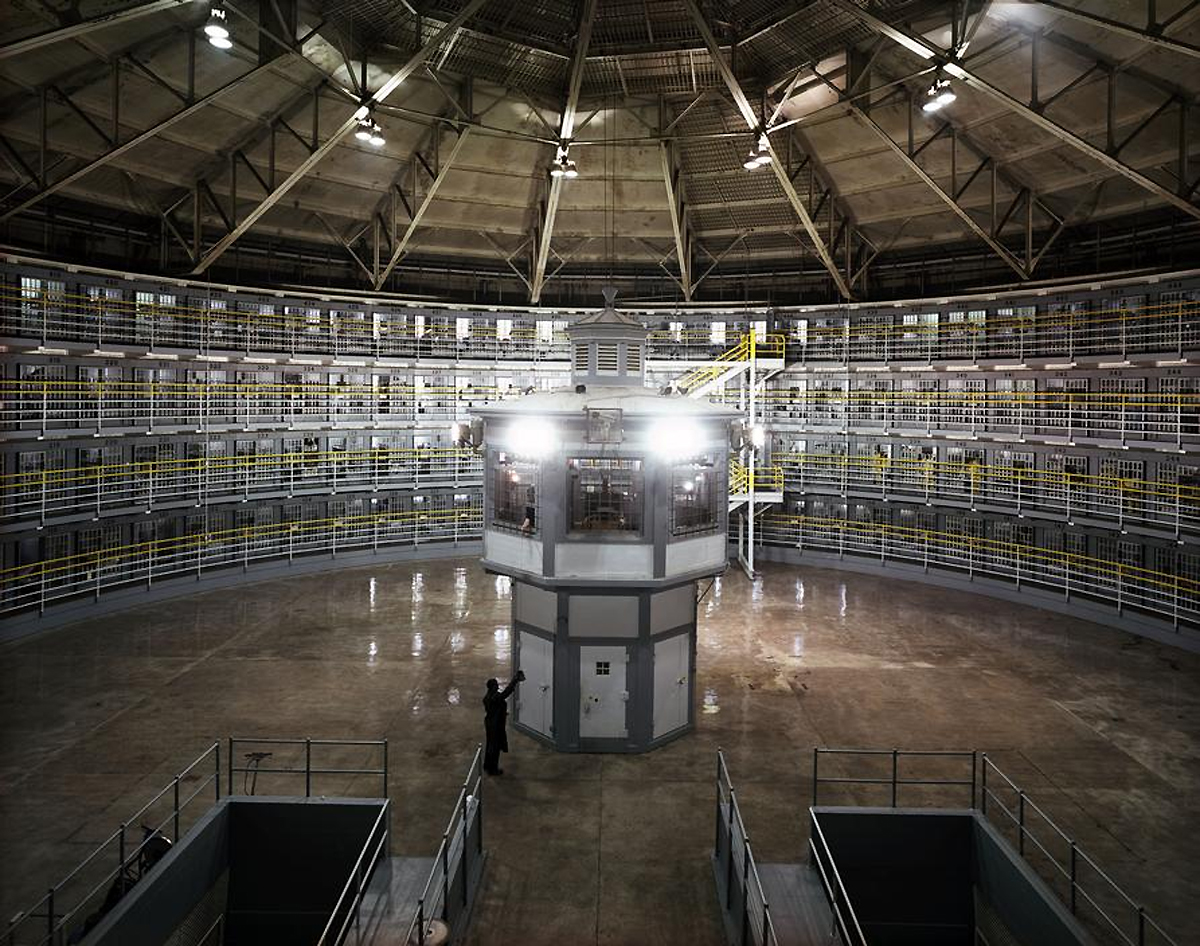
\includegraphics[width=350px]{chapters/01/images/panoptique.jpg}
    \caption{\label{panoptique} \emph{Stateville Correctional Center}, Illinois, États-Unis : Prison construite sur le modèle panoptique}
\end{figure}

\paragraph{} On retrouvera le panoptique dans la littérature de science fiction et d'anticipation du XX\up{ème} siècle.
Dans \emph{La Zone du Dehors} \cite{Damasio0}, Alain Damasio décrit une société désindividualisante qui, à la place
de noms, attribue des matricules changants à des citoyens normés. De manière à assurer \emph{préventivement} l'ordre et la
sécurité, des tours panoptiques aux parois de verre sans tain surplombent la cité et sont accessibles à tous pour épier
et reporter en toute impunité. Cela tend alors à développer chez chacun le sentiment latent et insidieux d'être observé, 
constamment sous surveillance.

\paragraph{} C'est justement sur cet effet que vont reposer, selon Michel Foucault, les nouveaux modèles disciplinaires.
\guillemotleft Le vrai effet du Panopticon, c'est d'être tel que, même lorsqu'il n'y a personne, l'individu dans sa
cellule, non seulement se croie, mais se sache observé, qu'il ait l'expérience constante d'être dans un état de visibilité
pour le regard. \guillemotright \cite{Foucault0} Dès lors, à quoi bon recourir à la violence ? Chacun se sachant, à tort
ou à raison, observé continuellement agira en conséquence. Mais Foucault pousse plus loin son raisonnement, comparant la
panoptique pénitentiaire à un système de documentation des individus. Le geôlier peut alors prélever sans interruption
des informations et observations à propos des détenus, les analysant, les catégorisant, dans le but de \guillemotleft 
[Faire] de la peine rendue nécessaire par l'infraction une modification du détenu, utile pour la société. \guillemotright

\paragraph{} Si l'on repense à la volonté initiale de Bentham d'appliquer le modèle panoptique à toutes sortes d'institutions
(universités, hôpitaux, ...), on assiste alors à l'objectification de l'individu, qui n'est plus considéré que comme le 
n\oe{}ud du complexe maillage qu'est la \emph{Société}, entité transcendentale se nourrissant de ses - ou plutôt de 
\emph{ces} ? - individus pour évoluer, pour le meilleur comme pour le pire.

\paragraph{} Mais de quoi les sociétés sont-elles consitutées sinon d'Hommes ? De là, ce sont bien les aspirations et 
motivations de ceux qui les composent qu'elles reflètent à l'identique, et c'est justement cette volonté de contrôle que
la technologie viendra par la suite outiller. Nous sommes bien loin de l'Oasis de Pierre Rabhi, pleine de paix et de
simplicité \cite{Rabhi1}. Nous allons donc d'abord nous intéresser à l'origine du Réseau, épine dorsale de nôtre Moi 
numérique, sans laquelle aucun des services que nous utilisons au quotidien n'aurait pu voir le jour.

\paragraph{} Les premières recherches ayant pour objectif la mise en place d'un réseau capable de résister à une frappe
nucléaire massive datent de 1957 \cite{Internet0}, quand le \emph{United States Department of Defense} (DoD) prend la
décision de fonder l'\emph{Advanced Research Projects Agency} (ARPA), un groupe scientifique ayant pour mission de concevoir
des innovations technologiques pour l'armée. Épaulés par les chercheurs de la \emph{RAND Corporation} à partir de 1962,
leurs travaux aboutiront un an plus tard sur l'ébauche d'un réseau décentralisé pouvant continuer à fonctionner dans le
cas où une ou plusieurs machines le composant viendraient à s'arrêter. L'idée d'un système décentralisé vient de Paul Baran,
qui inventa avec Donald Davies la communication de données par paquets, ajoutant ainsi à la résilience du système : le réseau
formant un maillage anarchique, chaque paquet pourra emprunter la route la plus courte possible afin de parvenir à sa 
destination, et aura la capacité de patienter durant un laps de temps maximal prédéfini s'il se trouvait dans l'incapacité
de la joindre.

\paragraph{} Le projet fut cependant refusé par l'armée, et il faudra attendre 1969, 6 ans plus tard, pour que celui-ci
se concrétise sous le nom d'\emph{Arpanet}. \emph{Bolt Beranek and Newman Inc.} (BBN) mettra en place, sur commande de
l'ARPA, un réseau reliant quatre des grands centres universitaires américains en utilisant le \emph{Network Control Protocol}
(NCP), sur des lignes pouvant atteindre 50 kilobits par seconde. Les universités concernées sont l'Université de Californie
à Los Angeles (UCLA), l'Institut de Recherche de Stanford (SRI), l'Université de Californie à Santa Barbara (UCSB) et
l'Université de l'Utah.

\begin{figure}[h]
    \centering
    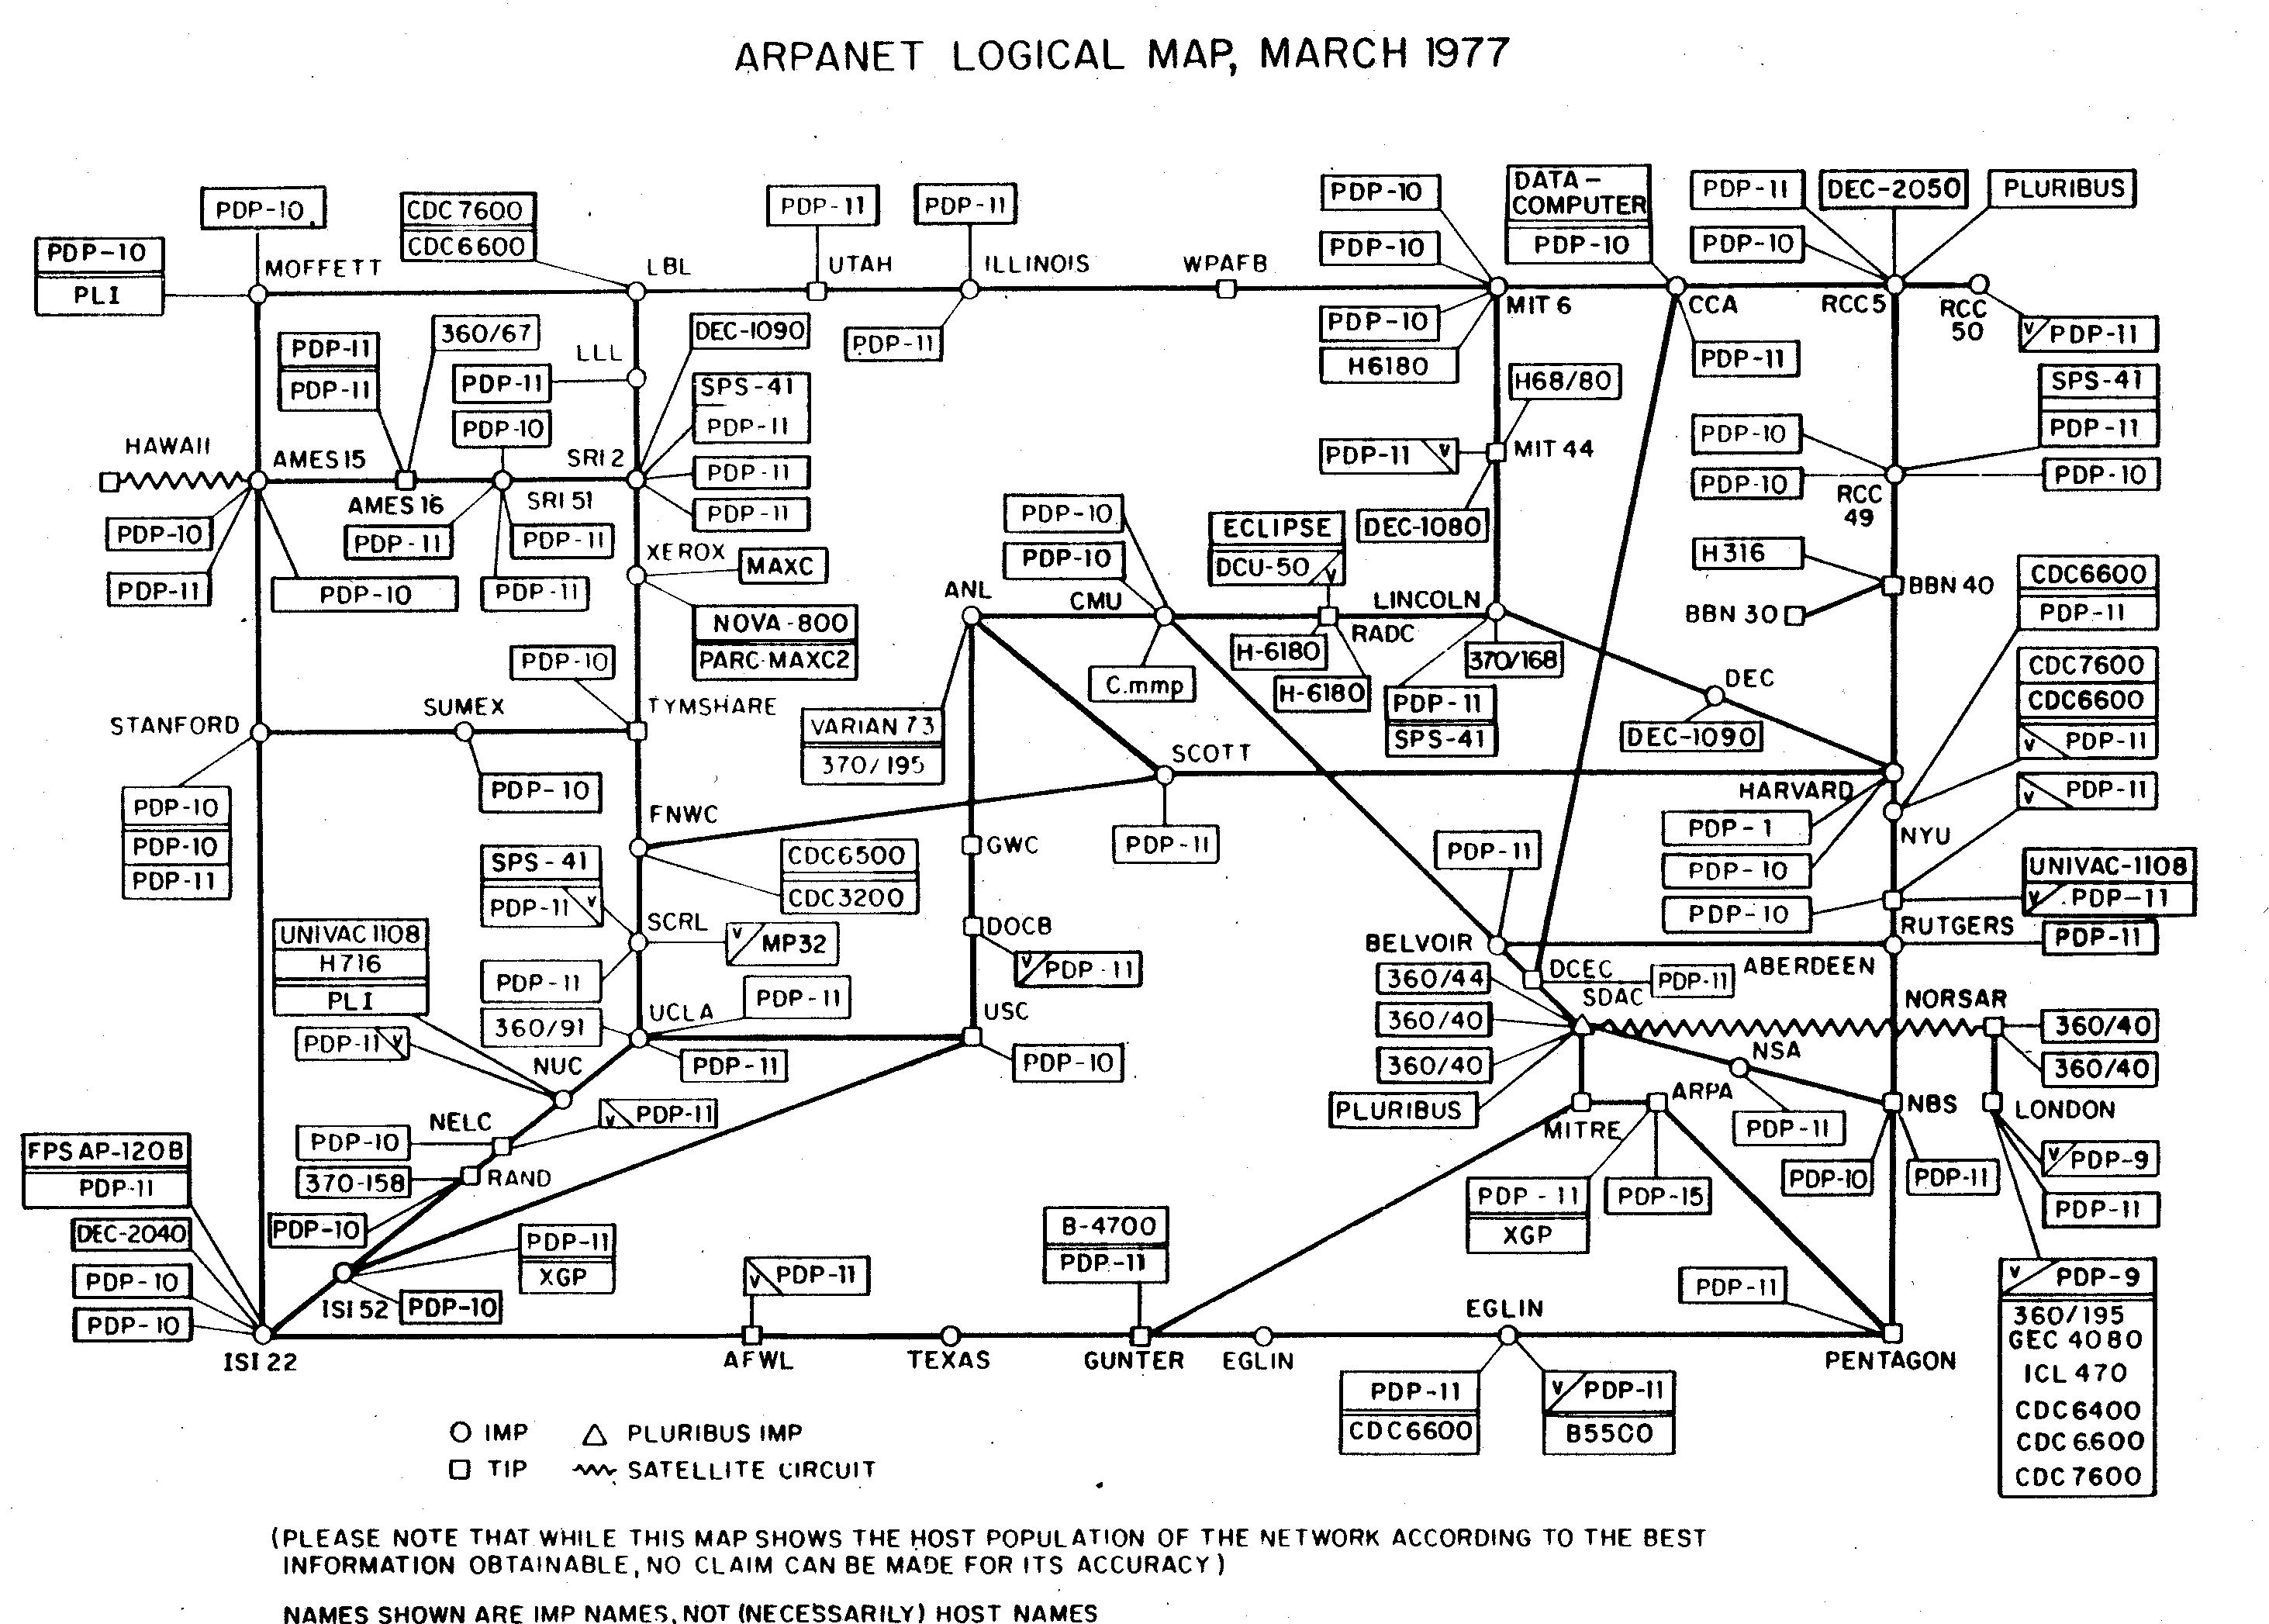
\includegraphics[width=400px]{chapters/01/images/arpanet_map.jpg}
    \caption{\label{arpanet} Carte du réseau Arpanet, mars 1977}
\end{figure}

\paragraph{} Il faudra attendre encore deux avancées majeures pour que ce réseau soit utilisable par le grand public :
le protocole TCP/IP, et le DNS.

\paragraph{TCP/IP} La suite TCP/IP, nommée après les deux premiers protocoles qui la compose (le \emph{Transmission Control
Protocol} et l'\emph{Internet Protocol}), est développée en 1973 par Vinton Cerf et Bob Kahn. Son modèle est constitué de
quatre couches prenant en charge la transmission de données : les couches hautes manipulent les données abstraites
présentées à l'utilisateur, tandis que les couches basses permettent la représentation de ces données sur un médium
physique (aujourd'hui : connecteurs 8P8C - abusivement appelés RJ45 -, fibres optiques, ...). Adopté pour l'Arpanet en
1976 sur décision du DoD, il faudra attendre 1983 pour sa mise en place effective.

\paragraph{Note} \emph{Serait-il pertinent de parler du modèle OSI ? Faire une comparaison entre les 7 couches OSI et les
4 couches IP, et expliquer pourquoi ce dernier n'a pas été retenu.}

\begin{figure}[h]
    \centering
    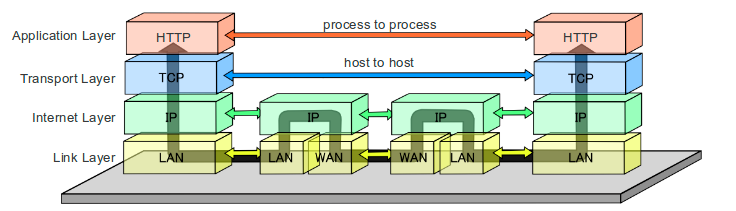
\includegraphics[width=400px]{chapters/01/images/tcpip_dataflow.png}
    \caption{\label{tcpip_dataflow} Flux de données du protocole TCP/IP}
\end{figure}

\paragraph{DNS} Le \emph{Domain Name System} (DNS) est la solution qui a été trouvée pour résoudre les problèmes survenus
suite à l'augmentation de la popularité du réseau Arpanet. En effet, de manière à ce que les différentes machines du 
réseau puissent communiquer entre elles, il était nécessaire qu'elles maintiennent à jour un fichier \emph{hosts.txt}
permettant d'effectuer la conversion entre un nom d'hôte et l'adresse correspondante sur le réseau. En réalité, ce fichier
était maintenu à jour par le \emph{Network Information Center} (NIC) de l'institut de recherche de Stanford, qui centralisait
les modifications qui lui étaient transmises par les différents administrateurs du système et qui s'occupait de redistribuer
périodiquement le fichier mis à jour. Cependant, avec l'augmentation progressive du traffic, le NIC se retrouva dans
l'incapacité de supporter la charge réseau et des problèmes de collision de nom survinrent de plus en plus fréquemment.

\paragraph{} Jon Postel, Paul Mockapetris et Craig Partridge rédigèrent donc 1983 les spécifications de ce qui devait 
devenir l'un des piliers d'Internet tel que nous le connaissons aujourd'hui : le DNS. Il s'agit d'une base de données
distribuée stockant les noms de domaines, et divisée en zones. Chacune de ces zones était prise en charge par un ou plusieurs
serveurs de noms (\emph{Name Servers}) répondant aux requêtes des résolveurs (\emph{resolvers}), petits programmes se
chargeant de transformer un nom de domaine en adresse. En 1984, les suffixes DNS, ou \emph{Top Level Domains} (TLD),
font leur apparition. Disposant chacun de leur propre zone DNS, ils permettront dans un premier temps de regrouper les
noms de domaine par fonction : \emph{.com} pour les sites commerciaux, \emph{.gov} pour les sites gouvernementaux des
États-Unis, etc. Avec le temps, certaines de ces particularités furent dépréciés (les sites en \emph{.com}
ne fournissent plus obligatoirement des services d'ordre commerciaux), et l'on vit apparaître les TLD nationaux (\emph{.fr},
\emph{.us}, \emph{.uk}, ...) dont l'obtention est soumise aux lois du pays concerné.

\paragraph{} Une fois ces systèmes mis en place, le réseau qui n'était à l'origine destiné qu'à des fins de recherche
militaire avait atteint un seuil majeur d'évolutivité. L'invention du "Web" est historiquement située en 1989 et
attribuée à Sir Timothy John Berners-Lee, alors chercheur au \emph{Conseil Européen pour la Recherche Nucléaire} (CERN)
de Genève, et à son texte \guillemotleft Information Management: A Proposal \guillemotright \cite{Internet1}. Sa volonté
est alors de mettre en place un système d'information global pour la recherche, à l'image d'Arpanet - mais accessible par tous.
Il est l'auteur d'\emph{httpd}, le premier serveur HTTP, et de \emph{WWW} (\emph{World Wide Web}), le premier client.
Il préside depuis 1994 le \emph{World Wide Web Consortium} (W3C), organisme qu'il a lui-même fondé et chargé de mettre
au point les nouveaux standards des technologies Web.

\paragraph{} Toutes les briques étaient en place pour l'adoption par le grand public : les technologies, réseaux comme
logicielles, étaient fin prêtes.

\section*{Brouillon}

\paragraph{Références} \cite{Marx0} \cite{Marx1} \cite{Nietzsche0}

\paragraph{Ère pré-internet} Analyse des dernières décénnies du XX\up{ème} siècle :
comment les sociétés ont évoluées avec l'arrivée des nouvelles technologies : du
pré-internet à l'ère des réseaux ; jusqu'à aujourd'hui. Quels étaient les objectifs
premiers des ces technos. (la raison de leur développement) ? Comment ont-elles réellement
été utilisées/ont été amenées à évoluer ? Est-ce réellement une mauvaise chose (n'y
a-t-il que du mal qui en soit ressorti) ? Est-il pertinent/nécessaire d'effectuer un bref
historique des technologies \emph{disruptives} (machine de Turing, architecture
Von Neumann, premiers réseaux, ...) ?

\paragraph{L'individu technique} Comment les modèles de sociétés nous ont-ils amené à
réfléchir l'individu en termes technologiques ?

\paragraph{Objectif} L'objectif ici est de démontrer que, suite au développement des technologies, c'est l'Homme
qui génère lui-même des données le concernant, par l'utilisation au quotidien des services (entre autres).
Cela doit être démontré par la mise en place d'un prototype récupérant des données de différents
services (ie facebook, twitter...)



\section*{Prototype}

\paragraph{} Pour étayer notre propos, un prototype servira de fil rouge tout au
long de votre lecture. Nous nous intéresserons ici à la récupération de données personnelles,
focus de cette première partie. Pour cela, nous avons restreint notre champs d'action à quelques
services pertinents pouvant nous apporter un maximum d'informations :

\begin{itemize}
    \item Facebook : récupération des données publiques des profils utilisateurs ;
    \item Twitter : récupération du profil et des derniers messages de l'utilisateur, jugés
    représentatifs de son \emph{opinion} ;
    \item Instagram : récupération des photos de l'utilisateur ; 
    \item Google Maps API : récupération des coordonnées géographiques associées à une adresse
    (\url{https://maps.google.com/maps/api/geocode/json?address={ADDRESS}}) ;
    \item Google : récupération des suggestions de pages liées à la personne concernée par le
    premier moteur de recherche mondial (\url{https://encrypted.google.com/search?q={SEARCH_TERMS}}) ;
    \item LinkedIn : récupération du profil professionnel de l'utilisateur (\emph{nécessite une clé d'API ?}).
\end{itemize}

\paragraph{} Afin de permettre une aggrégation simple de l'ensemble de ces données, une 
API REST sert de façade pour d'éventuelles applications ou un usage à des fins de recherche
par un être humain. La récupération concertée des informations concernant une personne peut
être effectuée grâce à une requête \lstinline{GET} sur l'URL \url{https://{API_URL}/people/{NAME}}
- la réponse est au format JSON.

\paragraph{} En arrière plan, plusieurs composants entrent en jeu. Pour chacun des services
ci-dessus, un \emph{récupérateur} dédié a la charge de l'obtention et du formatage des données
exposées. Ces différentes informations sont ensuite retravaillées et aggrégées de manière 
à créer un "\emph{profil utilisateur}" le plus complet possible à partir des informations
disponibles publiquement sur internet.

\paragraph{} Pour cette première version de notre prototype, aucun \emph{état} ni aucune
donnée ne sont persistés. Les \emph{endpoints} de notre API sont les suivants :

\begin{itemize}
    \item \url{/people/{NAME}}
    \item \url{/services/facebook/{NAME}}
    \item \url{/services/twitter/{NAME}}
    \item \url{/services/instagram/{NAME}}
    \item \url{/services/google/{NAME}}
    \item \url{/services/linkedin/{NAME}}
\end{itemize}
\section{L'irruption des technologies}
\paragraph{Références} \cite{Richesses0}

\paragraph{Collecter : hier et aujourd'hui}

\paragraph{} Le terme de \emph{collecte} n'est pas récent ; en effet il nous viendrait vraisemblablement
du XIVe siècle et du terme \emph{collete} en latin, qui signifie la \guillemotleft levée des impositions \guillemotright,
soit la période pendant laquelle un collecteur était en fonction. Cette définition relève de plusieurs notions
qui nous intéressent plus particulièrement.

\paragraph{} Tout d'abord, la collecte c'est la levée d'un impôt. C'est donc que le collecté \emph{doit}
quelque chose au collecteur, pour une \emph{raison} particulière : mise à disposition de biens, services,
protection... La collecte est donc un échange entre deux entités. Cet échange est avant tout un contrat de
pouvoir : contre tel service, en échange de tel accès, de telle reconnaissance, le collecté accepte de
léguer une part de ses biens, de ce qu'il est ou ce qu'il a. Ce qui n'est pas le cas du collecteur qui est
dans une situation de \emph{prêt}, car il ne pourrait pas, en effet, mettre à disposition un service dont
il ne contrôle pas le flux. Cela l'empêcherait de pratiquer sa \emph{condition de collecteur}, n'étant pas en
\emph{situation de force} par rapport aux collectés.

\paragraph{} Il y a donc un rapport de pouvoir entre collecteur et collecté. Le collecteur s'apparente à un n\oe{}ud
parent, qui exerce le même contrôle sur tous ses noeuds enfants, qui eux-mêmes ne peuvent finalement qu'accepter
le pouvoir émis par ce dernier, à partir du moment où il n'existe pas d'autre collecteur offrant le \emph{même
service} pour une \emph{peine moindre}. On reconnait là une première forme de centralisation des données.
Au départ, la collecte concerne évidemment les revenus, l'argent d'un foyer ou d'un particulier. Car cet
argent est le pouvoir de vie (ou de \emph{survie}) d'un Homme, il doit accepter d'en laisser, d'en léguer un peu
s'il souhaite avoir accès à un bien. Mais l'argent étant assez mal réparti au sein des sociétés \cite{Richesses0},
tous ne peuvent se permettre de payer. Ce sont alors d'autres biens qui sont collectés : récoltes, créations
artisanales... C'est le produit de la \emph{technique} de l'Homme qui est récolté. Ce sont son \emph{temps} et
ses \emph{capacités techniques} qui lui permettent de payer.

\paragraph{} Néanmoins, ces collectes demandent une contribution matérielle de la part du collecté, et ce n'est pas
nécessairement le cas. Un exemple ancien serait celui des citoyens, en Grèce antique, qui devaient être répertoriés
dans des tables afin de témoigner de leur condition de citoyen. A titre exceptionnel, des femmes ou des esclaves
devenaient parfois citoyen, et la présence de leur nom sur une tablette leur permettait de l'affirmer et d'être
reconnu comme tel. Un parallèle peut être fait avec l'exemple plus récent des nationalités et des cartes d'identité :
avoir un passeport ou une carte d'identité, c'est être citoyen d'un pays. C'est donc bénéficier des \emph{lois} de ce
pays quelque soit le cadre physique (ou presque). Dans les deux cas, le citoyen ne paie pas son recensement par de l'argent,
des récoltes ou autres. En revanche, il est \emph{de son devoir} d'être recensé, sinon il ne pourrait bénéficier des 
conséquences de son recensement. On peut alors statuer qu'il y a des récoltes de données qui sont \emph{indirectement
obligatoires} pour l'Homme bien qu'elles ne soient pas \emph{matériellement coûteuses}.

\paragraph{} La collecte est donc, qu'elle soit directe ou indirecte, \emph{imposée}. Dans nos exemples précédents,
la collecte est toujours \emph{acceptée} et \emph{consciente}. Acceptée tout d'abord car il n'y a finalement pas le
choix : si je souhaite bénéficier de quelque chose, je dois pouvoir céder une contrepartie. C'est la nature même des
échanges humains - je ne suis prêt à te donner ceci qu'\emph{en échange de} cela. Il y a donc une interaction directe 
: deux humains intéragissent pour parvenir à un accord. Mais ce n'est justement que parce que cette collecte met en
jeu deux humains qu'elle peut être qualifiée de \emph{consciente} - parce que le collecté est capable de se dire à
un instant précis qu'\emph{il est effectivement en train de céder la contrepartie} à quelque chose. Ce n'est pas
toujours le cas et c'est pourquoi nous devons distinguer deux formes particulières d'acceptation de la collecte :
\emph{consciente} et \emph{inconsciente}.   

\paragraph{Collectes et consciences} \label{collect_data_conscious}

\paragraph{} Avant même de parler de conscience de la collecte, il est de bon ton de rappeler,
comme le précise C.G. Jung, qu' \guillemotleft Il est assez stérile d'étiqueter les gens et de les presser dans
des catégories \guillemotright. Par ici, on entend que l'\emph{expérience} même de la conscience est différente
pour tout un chacun. On parlera donc de "collecte affirmée" pour ce qui est conscient, et de "collecte non précisée"
pour ce qui est inconscient. Tout le monde n'est pas conscient que les publicités que l'on voit sur internet sont
ciblées ; et même si les utilisateurs y sont de plus en plus attentifs, il n'est pas indiqué à côté de chaque
publicité "Cette pub pour tel achat est présente car nous avons collecté vos dernières recherches et que plus d'un
quart concerne ce sujet ou des sujets proches". 

\paragraph{} Tout ce qui est inconscient est plus évident à aborder en premier lieu pour une raison simple : tout est
inconscient par définition. Prendre conscience de, c'est \emph{considérer} quelque chose, y porter \emph{son attention}.
Or, par nature, l'Homme ne porte attention qu'à une chose à la fois, et certainement pas à l'ensemble de son
environnement. Toute donnée doit donc, dans l'absolu, être collectée de façon inconsciente : de l'heure du réveil au
temps mis pour se préparer, l'itinéraire choisi pour aller au travail ou faire des courses, les lieux et les personnes
qui ont été fréquentées... L'ensemble des données générées au quotidien par tout être humain est collectable par
définition. Les questions qui se posent donc sont : comment, et quelles données sont pertinentes ?

\paragraph{} Afin d'apporter une réponse à la première question il est important de s'arrêter un instant sur le fait
suivant : lorsque l'on rend la collecte \emph{nécessaire pour le collecté} - comme dans l'exemple précédent sur la
citoyenneté - elle n'est plus \emph{inconsciente}, car elle est \emph{affirmée}. La nécessité de la collecte porte
l'attention du collecté sur cette dernière, qui devient alors par définition \emph{consciente}. Cela
implique donc qu'une collecte est \emph{inconsciente} uniquement si elle \emph{ne créé par de nécessité}
chez le collecté. On se rend alors immédiatement compte que c'est l'arrivée de nouvelles techniques et de la
technologie qui permet une collecte de données \emph{inconsciente}. En s'infiltrant dans les interstices de nos vies -
smartphone, ordinateur, internet, transports, paiements - la technologie \emph{traque tout} et \emph{tout le temps},
sans que nous ne nous en aperçevions. Une évolution importante de nos jours, et que nous détaillerons par la suite, est
celle de l'IoT (Internet of Things) et des objets connectés en général. Leur utilisation permet une collecte plus
poussée mais surtout \emph{plus proche} de l'utilisateur, et donc une récolte de données bien plus \emph{précise}. Or
nous verrons lorsque nous aborderons le thème du Machine Learning qu'il existe un lien fort entre la précision d'une
donnée et la qualité du service qui pourra être fourni à un utilisateur (voir \ref{select_data_ml}).

\paragraph{} Puisque ces données sont partout, et qu'elles vont être de plus en plus récupérées, il est devenu
une question importante que celle du \emph{stockage} de ces données. Afin d'optimiser ce stockage, et avant même de
penser aux techniques physiques utilisées pour garder des données, il faut effectuer un tri dans ce qui sera récupéré.
Pourtant, ce tri est aujourd'hui davantage effectué une fois que la donnée est récupérée. En effet, afin de déterminer
si une donnée est pertinente, il suffit de se demander si elle apporte des informations suffisantes à la récupération
d'un bénéfice futur. C'est le principe même de \emph{collecte} : le collecté consomme et le collecteur en tire \emph{
une valeur}, directe ou indirecte. C'est donc bien qu'il y a une question de \emph{monétisation} de la donnée. La
problématique n'est plus donc de savoir quoi récupérer mais plutôt de comment exploiter ce qui à été récupéré.

\paragraph{} Dès lors que nous parlons de création de valeur, cela replace le contexte de la collecte dans un échange
\emph{conscient}, ou plutôt \emph{affirmé}, de la donnée. Il faut au départ que le collecteur produise un \emph{service},
qu'il existe un \emph{contrat} entre collecteur et collecté pour que la création de données ait lieu. Une matérialisation
simple et actuelle de cela se retrouve lorsqu'un utilisateur installe une application sur son smartphone - il est
alors invité à accepter ou non que l'application ait à son tour accès à un certain nombre de choses (medias, gallerie,
données personnelles, agenda...) sur le smartphone. C'est la partie \emph{consciente} du choix. Une fois qu'elle est
\emph{acceptée}, la partie \emph{inconsciente est alors acceptée également par défaut}. En effet le collecté accepte que
l'utilisation qu'il va faire de l'application soit collectée \emph{de facto}, par la \emph{nécessité d'accès à un service}.

\paragraph{Prototype}

\paragraph{} Pour étayer notre propos, un prototype servira de fil rouge tout au long de votre lecture : \lstinline{Tomorrow}
(\url{https://github.com/tomorrow-paper}). Nous détaillerons à la fois les objectifs remplis par chacun de ses modules
ainsi que les choix techniques que nous avons effectués.

\paragraph{TODO} \emph{Est-il nécessaire de préciser que nous utilisons le langage Rust et de justifier ce choix ici ?}

\paragraph{} Pour accompagner ce premier chapitre, nous avons souhaité mettre en place un service permettant d'aggréger
des données depuis n'importe quelle source pour ensuite pouvoir les consommer de manière normalisée.
Nous nous intéresserons ici à la récupération de données personnelles, et avons donc pour cela restreint notre champs
d'action à quelques services pertinents :

\begin{itemize}
    \item Google : récupération des suggestions de pages liées à la personne concernée par le
    premier moteur de recherche mondial (\url{https://encrypted.google.com/search?q={SEARCH_TERMS}}) ;
    \item Google Maps API : récupération des coordonnées géographiques associées à une adresse
    (\url{https://maps.google.com/maps/api/geocode/json?address={ADDRESS}}) ;
    \item Facebook : recherche et récupération des données publiques des profils utilisateurs
    (\url{https://www.facebook.com/public/{PEOPLE}}).
\end{itemize}

\paragraph{} De manière à préserver la séparation des responsabilités des composants de notre prototype, plusieurs modules
ont été développés : 

\begin{itemize}
    \item \lstinline{tomorrow-core} (\url{https://github.com/tomorrow-paper/tomorrow-core}) : contient la logique et les
    structures de données communes à tous les composants du prototype (gestion d'erreur, type résultat, ...) ;
    \item \lstinline{tomorrow-http} (\url{https://github.com/tomorrow-paper/tomorrow-http}) : contient les interfaces et
    implémentations la logique de requêtage à travers le protocole HTTP.
    \item \lstinline{tomorrow-recuperator} (\url{https://github.com/tomorrow-paper/tomorrow-recuperator}) : contient les interfaces
    de récupération de données.
\end{itemize}

\paragraph{} Ce découpage n'est pas anodin. Il nous permet par exemple de développer, pour chaque service cible, un module
dédié implémentant les interfaces définies dans \lstinline{tomorrow-recuperator}  :

\begin{lstlisting}
use tomorrow_core::Result;

pub trait Request {}
pub trait Response {}

pub trait Recuperator<Req, Res> where Req: Request, Res: Response {
    fn compute(&self, request: Req) -> Result<Res>;
}\end{lstlisting}

\paragraph{} Ces différents \emph{récupérateurs} sont ensuite utilisés pour constituer un composant à plus haut niveau
d'abstraction : \lstinline{tomorrow-api} (\url{https://github.com/tomorrow-paper/tomorrow-api}). API REST produisant des
documents JSON, elle sert de façade pour d'éventuelles applications ou un usage à des fins de recherche par un être humain. 
Pour cette première version de notre prototype, aucun \emph{état} ni aucune donnée ne sont persistés. Les informations 
sont lues à un instant \emph{T} quand l'utilisateur en fait la demande et lui sont immédiatement renvoyées par l'API.
Les \emph{endpoints} actuels sont les suivants (tous les modules peuvent être trouvés sur notre dépôt) :

\begin{itemize}
    \item \url{/services/maps/{ADDRESS}} : Google Maps grâce au module \lstinline{recuperator-google-maps} ;
    \item \url{/services/search/{QUERY}} : Google Search grâce au module \lstinline{recuperator-google} ;
    \item \url{/services/facebook/public/{PEOPLE}} : Facebook Public Search grâce au module \lstinline{recuperator-facebook}.
\end{itemize}

\paragraph{} Nos objectifs en développant ce service étaient triples. Tout d'abord, il se devait d'être agnostique en terme
d'utilisation : une API REST ne repose que sur le protocole HTTP, et le format JSON est aujourd'hui un standard en terme
d'encodage d'information. Ensuite, nous souhaitions l'architecturer de manière évolutive : pour récupérer les données
depuis un nouveau service, il suffit de créer un module implémentant les interfaces \lstinline{tomorrow-recuperator} et
de l'intégrer à l'API derrière un nouvel \emph{endpoint}. Enfin nous espérons qu'il vous aidera à prendre conscience que
rien n'empêche l'exploitation d'une donnée accessible publiquement sur Internet de nos jours. Car peu importe le nombre
de services différents que nous pourrions intégrer à ce prototype : c'est sa nature même qui doit vous interpeler.
\section{Les sociétés de contrôle}

\paragraph{Une portée personnelle}

\paragraph{} L'utilisation d'un service est de nos jours synonyme de production et donc collecte de données ; ne dit-on
pas que si un service est gratuit, c'est que ses utilisateurs en sont les produits ? Dès lors nous ne sommes plus maîtres
des informations que nous publions, qui peuvent être vendues ou récupérées à des fins diverses : publicité et marketing
ciblés en sont des exemples bien connus.

\paragraph{} Mais les données ne sont pas uniquement utilisées de manière ciblée. Le développement ces dernières années 
des \emph{Smart Cities} donne naissance à des initiatives auparavant impensables. Ainsi la ville de New York s'est-elle
dôtée d'un tableau de bord \cite{ProgrammableCity1} aggrégeant l'ensemble des sources de données à sa disposition pour 
mettre en exergue de nombreux indicateurs : fluctuation des prix de l'immobilier, évolution du nombre de plaintes pour 
tapage nocturne par quartier, hygiène des rues, état de la circulation aux différentes heures de la journée...
Toutes ces données dont \emph{nous} sommes la source sont ainsi mises au service de la ville.

\paragraph{} \emph{The Programmable City} \cite{ProgrammableCity0} est un projet proposant de mettre la technologie au
service de l'urbanisme. Une infrastructure et un ensemble de programmes nous permettent de piloter et d'être à l'écoute
de la ville, qui bénéficie au quotidien d'une attention nouvelle : on crée alors un cercle vertueux. Le site
\url{http://DublinDashboard.ie/} est une mise en application de ces concepts pour la ville de Dublin, proposant des
dizaines de sources de données visualisables concernant l'agglomération. D'autres initiatives, comme celle de SideWalk Labs
à Toronto \cite{ProgrammableCity3}, visent à réinventer la ville pour remettre l'humain au c\oe{}ur des processus de
décision en utilisant les nouvelles technologies et les données générées pour améliorer de manière continue les services
qu'elle fournit.

\begin{figure}[h]
    \centering
    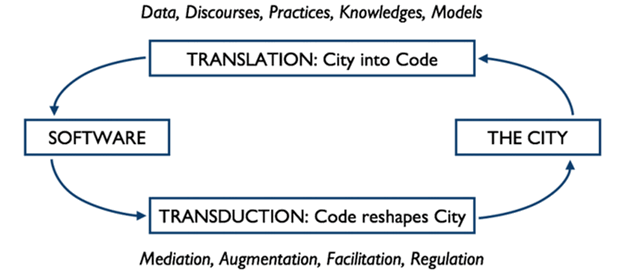
\includegraphics[width=300px]{chapters/01/images/programmable_city.png}
    \caption{\label{programmable_city} Le cycle de transduction des \emph{Programmable Cities}}
\end{figure}

\paragraph{} Une donnée, ce n'est rien de plus que de l'information numérisée. Là où ces bases de données publiques
émanant de structures privées ne nous étonnent en rien - car nous sommes \emph{habitués} à les alimenter, comme l'application
Uber Movement permettant d'analyser les trajets effectués via le service Uber -, il est important de comprendre
qu'elles ne diffèrent pas de celles de nos services publics. Ce n'est qu'avec l'adoption progressive de l'\emph{Open
Data} que ces derniers se sont petit à petit ouverts au développement d'applications exploitant toutes sortes de données. 

\paragraph{} Bien évidemment, les \emph{Open Data} et autres sources de données des \emph{Smart Cities} ne sont pas
constituées de données personnelles - c'est à dire d'informations permettant d'identifier de manière directe ou non une 
personne physique \cite{PersonalData0}. Mais cela est-il réellement différent ? Ainsi la société Hitachi a-t-elle développé
en 2015 un système de prévention des crimes et délits reposant sur du machine learning \cite{ProgrammableCity2}. Une quantité
astronomique de données de toutes sortes est nécessaire pour alimenter le système, des mouvements de population aux 
antécédents de crimes enregistrés dans les zones sous surveillance. Ne peut-on pas alors craindre de voir une zone 
démographique désertée suite à un incident car son \emph{coefficient de criminalité} aura augmenté, rebutant nouveaux
résidents et jeunes parents à s'y installer ?

\paragraph{} La finalité de ces systèmes peut être réduite à cette simple question : se savoir surveillé restreint-il
les instincts pervers, ou au contraire cela les désinhibe-t-il ?

\paragraph{} \emph{Veiller} nous vient du latin classique \emph{vigilare} \guillemotleft être éveillé, être attentif, sur
ses gardes \guillemotright, mais aussi \guillemotleft entourer de soins \guillemotright \cite{Surveillance0}. Le préfixé
\emph{Surveiller} (XVI\up{ème} siècle) signifie alors \guillemotleft contrôler, observer avec attention \guillemotright.
Être \emph{sous la surveillance de}, c'est être \emph{observé par} mais aussi \emph{contrôlé par}, c'est-à-dire subordonné
directement ou indirectement à quelquechose ou quelqu'un.

\paragraph{} L'\emph{instinct} vient du latin \emph{instinctus}, qui dispose d'un double sens. En latin classique, il 
signifie \guillemotleft instigation, excitation, impulsion \guillemotright, et en latin chrétien \guillemotleft penchant,
tendance naturelle \guillemotright \cite{Instinct0}. Théorisé par les philosophes, le mot désigne pour Montaigne (XVI\up{ème} siècle) 
\guillemotleft l'ensemble des pulsions naturelles qui régissent le comportement animal ou humain \guillemotright (cette 
notion de \emph{pulsion} se retrouve chez Freud avec le \emph{Trieb} allemand), tandis que Pascal (XVII\up{ème} siècle)
en fait \guillemotleft la faculté naturelle de sentir, de deviner \guillemotright.

\paragraph{} Enfin, \emph{pervertir} apparaît dans l'ancien français au XII\up{ème} siècle sous la forme \emph{purvertir} et est
dérivé du latin \emph{pervertire} ; \emph{per-} \guillemotleft l'action de \guillemotright, et \emph{vertere} \guillemotleft
tourner, verser \guillemotright : il signifie alors \guillemotleft mettre sens dessus-dessous, faire mal tourner \guillemotright
\cite{Pervers0}. Dans le langage religieux, le \emph{pervers} est une personne \guillemotleft portée à faire le mal \guillemotright
et est alors synonyme de \emph{dur}, \emph{cruel}, \emph{furieux} (XIII\up{ème} siècle). En français moderne, il désigne 
\guillemotleft la personne qui montre une tendance pathologique à accomplir des actes immoraux \guillemotright, voire même
celle \guillemotleft dont les \emph{pulsions} ne sont pas fixées \guillemotright pour les psychanalystes.

\paragraph{} Qu'entend-on donc par \emph{instincts pervers} ? L'instinct, c'est la pulsion ; la perversion, c'est l'absence
de fixation. Or \emph{fixer}, c'est \guillemotleft établir d'une manière durable dans une position déterminée \guillemotright \cite{Fixe0}.
Les instincts pervers, ce sont donc toutes les pulsions "hors norme", hors du cadre déterminé, en décalage avec la réalité
telle qu'elle est acceptée (ou définie) par le groupe ; la perversion n'a de sens que dans un contexte sociétal.

\paragraph{} Nous touchons donc bien à la raison d'être des sociétés de contrôle : restreindre les instincts pervers c'est
normaliser, niveller par le bas, et l'ensemble des systèmes de surveillance contribuent à accentuer ce phénomène \cite{SocialMedia0}.
\emph{Se savoir surveillé}, ce n'est rien de plus que posséder un compte sur un réseau social : on y incarne à tour de
\emph{rôle} juge, avocat et accusé, et l'on s'accroche à l'idée illusoire que l'on n'a pas perdu le \emph{contrôle}.

\paragraph{} Vaudrait-il mieux alors vivre dans une société où sévissent quelques individus extrêmement pervers, ou dans
une société \emph{lissée}, \emph{amortie}, \emph{normalisée} ? Le modèle panoptique (voir \ref{panoptique}, page \pageref{panoptique})
ne s'est jamais généralisé car il était trop évident, manquant de subtilité. Les technologies ont permis de mettre en application
le modèle du \emph{surveilleur-surveillé}.


\paragraph{Évolution du partage}

\paragraph{} Évolution du partage : les réseaux sociaux, quelles moeurs ? Catégoriees d'âges ? Sociaux-professionnelles ?
Quelle forme de contrôle incarnée par notre prototype ? À qui est-il destiné ? Pour quelles utilisations ?
La place de l'information/désinformation ?


\paragraph{L'individu technique}

\paragraph{} Comment les modèles de sociétés nous ont-ils amené à réfléchir l'individu en termes technologiques ? 

\chapter{Un Système pour les gouverner tous}
\paragraph{Objet} Systèmes possibles ; Réseau Distribué
\paragraph{Technique} Un système distribué : scalabilité et résilience applicative
\paragraph{Références}
\cite{Deleuze:0}
\cite{Foucault:0}
\cite{Negri:0}
\cite{Pieces:0}
\cite{ProgrammableCity:0}
\cite{ProgrammableCity:1}
\cite{PsychoPass}

L'objectif ici est de mettre en place un prototype qui se chargera de la récolte des données
de manière insidieuse et de leur mise ne réseau. Un logiciel, installé sur un ou plusieurs pc,
pourra envoyer des données à une entité centrale ou bien échanger entre eux.

\section{Un Réseau}
\paragraph{Références} \cite{DarkWeb:0}

\paragraph{Réseau \emph{nominal}} "Idéal" de la mise en place d'un Réseau universel, omniprésent
et omniscient. Un tel système global impliquerait la mise en place d'un système hautement
distribué, voire \emph{"participatif"}.

\paragraph{Réseaux parallèles} Verra-t-on un jour la disparition des réseaux parallèles
(TOR, blockchains, ...) ? Ces technologies \emph{disruptives} seront-elles un jour vouées
à disparaitre ou au contraire à se développer avec d'autant plus d'ardeur ? Peut-on alors
parler d'une neutralisation du Réseau par le réseau ?


Do it Yourself : Mettez en place votre propre télémétrie ! (Keylogger ?)

\section{Des contraintes architecturales}
\paragraph{Des contraintes à prendre en compte} Scalabilité, résilience..
\paragraph{Vecteurs d'adhésion} OS, Suprématie Windows/OSX

Attention aux redites - le but ici est de montrer que l'Homme est à la fois
consommateur et producteur des informations transitant sur le réseau.

\section{L'Homme gouverne l'Homme}
\paragraph{Références} \cite{GhostInTheShell}

\paragraph{Un rêve devenu réalité ?} Systèmes distribués, mise en oeuvre à grande échelle.
À travers le Réseau, c'est l'Homme qui devient omniscient.

\paragraph{L'Homme} Chaque foyer comme noeud du réseau, chaque individu comme neurone du
système. La surveillance n'est pas \emph{automatique}, le système ne s'auto-alimente pas :
c'est à travers \emph{nos} interactions qu'il se nourrit et prend de l'ampleur (ajout de 
contenus, d'informations de plus en plus exhaustive sur nous et nos connaissances, ...).
\chapter{L'intelligence envahissante de votre quotidien}
\paragraph{Objet} Développement technique
\paragraph{Technique} Intelligence, traitement des données
\begin{itemize}
    \item Tendances actuelles
    \item prévisions
    \item Analyses psychologiques
    \item Géolocalisation
\end{itemize}

\paragraph{Références}
\cite{Asimov:0}
\cite{Moore:0}
\cite{MachineLearning:0}
\cite{MachineLearning:1}
\cite{ProgrammableCity:0}
\cite{ProgrammableCity:1}
\cite{GhostInTheShell}
\cite{PsychoPass}


\section{Intelligence as a Service}
\paragraph{Références} 

\paragraph{Qu'est-ce que l'IA ? Quelle est sa place ?} Nous entendons parler
de plus en plus d'intelligence artificielle, mais quels sont ses principes
fondateurs ? Comment ce domaine s'est-il démocratisé ? Quels exemples avons-nous
de son utilisation dans des systèmes actuels ? 

\paragraph{Quelles contraintes ?} Quelles sont les conditions techniques nous
permettant d'intégrer de l'IA dans des systèmes ? Y a-t-il des contraintes de
volumétrie, de scalabilité, de puissance de calculs ? Nous verrons comment
l'intégration de systèmes intelligents s'est faire avec plus ou moins de succès
selon et les projets, ainsi que les solutions et évolutions qui ont été apportéées,
permettant de simplifier la mise en place et l'utilisation d'IAs. 

\paragraph{Quels apports et quelle utilité ?} Quels sont les apports \emph{concrets}
de l'IA ? Quels domaines sont les plus concernés ? Est-il possible de distinguer
des \emph{patterns d'implémentation} permettant d'apporter des réponses systématiques
à des problèmes connus ?

\paragraph{Objectif} L'objectif est d'ajouter ici des traitements de données automatisés au section
du Réseau.

\section{Machine Learning}
\paragraph{Références} \cite{AlphaGo:0} \cite{AlphaGo:1}

\paragraph{Différences et similitudes avec IA} En quoi consiste le ML ? Bien qu'il soit
directement lié à l'IA, quelles sont ses différences et ses similitudes avec cette dernière ?

\paragraph{Evolution logique et inévitable de l'IA} 

\paragraph{Systèmes intelligents} Lorem ipsum


\section{Usages, dérives et éthique}
\paragraph{Références} \cite{Asimov:0} \cite{Damasio:0}

\paragraph{Déterminisme, cas d'utilisations} Lorem ipsum

\paragraph{Eugénisme, dérives} Lorem ipsum

\paragraph{Améliorations de vie et sociales} Lorem ipsum
\chapter{Conclusion}

\paragraph{} C'est donc chaque jour que nous délaissons notre puissance au profit des
technologies. A travers Internet, les smartphones, les objets connectés, nous acceptons
à chaque instant de \emph{léguer} et de \emph{déléguer} une part de nous-même à la 
technologie. 

\paragraph{} Allégorie du contrôle, propre de l'Homme, les données que ces
interactions génèrent sont \emph{traquées partout et tout le temps}, et les quantités
gigantesques que cela représente dépassent maintenant l'entendement. Ces données sont
générées par l'Homme \emph{à chaque instant}, sans plus \emph{aucune interruption}. 

\paragraph{} L'individu se conceptualise en termes technologiques. Il est devenu un
individu technique, \emph{un profil}. L'image que l'on cherche à donner à travers la
technologie ne reflète que celle que l'on souhaite adopter. Et au-delà \emph{du Moi}
qui est devenu le centre des intérêts, l'Homme reste à la fois \emph{connecté} mais
\emph{paradoxalement seul}.

\paragraph{} Seul, il constitue un des noeuds du réseau \emph{omniprésent} que représente
déjà internet. Et il en est \emph{l'acteur principal} : c'est sa projection à travers
les services \emph{qu'il créé et qu'il utilise} qui va former \emph{son Moi technologique}.

\paragraph{} Et ces services forment eux-mêmes des réseaux par leurs interconnexions : la facilité
d'accès est avant tout centrée \emph{sur l'utilisateur}. Mais cette facilité n'est qu'une interface
\emph{créée par le facilitateur} pour servir ses propres intérêts. Ainsi les services se doivent
d'évoluer vers \emph{un écosystème commun} s'ils souhaitent asseoir leur \emph{universalité},
non au détriment \emph{de l'individu}. 

\paragraph{} Mais l'Homme s'est toujours gouverné lui-même. En société ou seul, il se fixe
\emph{des règles}, qui lui permettent d'évoluer, de se fixer un objectif, \emph{d'avancer}.
Ce comportement est le propre de l'Homme, et est une conséquence directe de son intelligence.
En choisissant de la déléguer \emph{aux machines}, il choisit de déléguer aussi
bien une partie du contrôle qu'il exerce \emph{sur lui} que de celui qu'il exerce \emph{sur autrui}.

\paragraph{} C'est donc \emph{aux systèmes} que le contrôle est délégué, et nous qualifions
nous-même ces systèmes \emph{d'intelligents}. Embarquée partout : smartphones, transports,
médical, finance, robotique ; l'Intelligence Artificielle est un formidable vecteur
\emph{de découvertes}. La puissance des IA à longtemps été fantasmée, et pourtant 
certaines \emph{dépassent} maintenant l'Homme dans des problèmes d'une complexité \emph{infinie}. 

\paragraph{} Le Machine Learning en est l'exemple le plus marquant des dix dernières
années. En reproduisant le fonctionnement \emph{du cerveau de l'Homme}, les machines sont
arrivées à faire ce qui était alors impossible : \emph{apprendre}. Et leur apprentissage
dépasse les attentes humaines, aussi bien dans la vitesse de progression que dans la
\emph{réelle application technique}. Cette avancée technologique se cristallise et 
atteint son paroxysme à travers les dernières découvertes du machine learning : la
machine apprend \emph{mieux, sans l'aide de l'Homme}. 

\paragraph{} Toutes les dérives négatives, scenarii catastrophe issus de notre imagination,
sont déjà \emph{à portée de main}. Les données sont \emph{accessibles}, les réseaux \emph{universels},
les machines \emph{humanisées}. Il ne tient qu'à une société, un état, un
individu, de choisir \emph{la manière} de laquelle il souhaite \emph{utiliser et être
utilisé par} ces outils.

\paragraph{} La balle est donc dans \emph{notre camp}, nous êtres humains. Quel sera
notre choix pour la société de demain ? Il ne tient qu'à nous de saisir
l'opportunité de l'élan technologique pour \emph{créer, aider}, et inventer
intelligemment notre espace virtuel et réel de demain. Mais la dissociation entre
les deux est encore mal faite, car nous ne sommes que \emph{les premières générations}
à être confrontés à de tels enjeux. Il s'agit maintenant de trouver des techniques
\emph{non-intrusives}, permettant de concilier \emph{innovation bénéfique} et
respect de \emph{l'individualité}.

\paragraph{} Cependant rien ne nous dit qu'il n'existera pas, demain, un \emph{système pour nous
gouverner tous}.

\pagenumbering{roman}

\chapter{Annexes}

\section{Chronologie}
\label{chronology}

\begin{itemize}
    \item 1957 : Création de l'\emph{Advanced Research Project Agency} (ARPA) par le \emph{Department of Defense} (DoD) des États-Unis ;
    \item 1962 : Invention d'un réseau décentralisé et de la communication de données par paquet par Paul Baran et Donald Davis ;
    \item 1969 : Concrétisation de leur projet sous la forme du réseau \emph{Arpanet} ;
    \item 1973 : Invention du \emph{Transmission Control Protocol} (TCP) et de l'\emph{Internet Protocol} (IP) par Vinton Cerf et Bob Kahn ;
    \item 1976 : Adoption du protocole TCP/IP pour l'Arpanet par le DoD ;
    \item 1983 : Mise en place effective de la suite TCP/IP sur Arpanet ;
    \item 1983 : Invention du \emph{Domain Name System} (DNS) par Jon Postel, Paul Mockapetris et Craig Partridge ;
    \item 1984 : Invention des \emph{Top Level Domains} (TLD) ;
    \item 1989 : Invention du \emph{World Wide Web} par Sir Timothy John Berners-Lee ;
    \item 1994 : Fondation du \emph{World Wide Web Consortium} (W3C) par Sir Timothy John Berners-Lee.
\end{itemize}
\begin{thebibliography}{99}
    \bibitem{23andMe} \emph{23andMe}, \url{https://www.23andme.com/howitworks/}

    \bibitem{AI0} Artificial Intelligence, \url{https://en.wikipedia.org/wiki/Artificial_intelligence}
    \bibitem{AI1} Virginie Mathivet, \emph{L'Intelligence Artificielle pour les développeurs Java}, eni Editions, 2015
    \bibitem{AI2} John McCarthy, \emph{Biography}, \url{http://www.computerhistory.org/fellowawards/hall/john-mccarthy/}

    \bibitem{AlphaGo0} David Silver \and Aja Huang, \emph{Mastering the Game of Go with Deep Neural Networks and Tree Search}, 2016, \url{https://gogameguru.com/i/2016/03/deepmind-mastering-go.pdf}
    \bibitem{AlphaGo1} Mirek Stanek, \emph{Understanding AlphaGo}, 2017, \url{https://machinelearnings.co/understanding-alphago-948607845bb1}
    \bibitem{AlphaGo2} AlphaGo Zero: Learning from scratch, \url{https://deepmind.com/blog/alphago-zero-learning-scratch/}
    \bibitem{AlphaGo3} Seth Weidman, \emph{3 tricks that made AlphaGo Zero work}, \url{https://hackernoon.com/the-3-tricks-that-made-alphago-zero-work-f3d47b6686ef}

    \bibitem{Arte0} \emph{Informations, le grand complot}, Arte, 2017, \url{https://www.arte.tv/fr/videos/074592-000-A/informations-le-grand-complot/}, \url{https://www.youtube.com/watch?v=RfybAOSlrSs}

    \bibitem{Asimov0} Isaac Asimov, \emph{Fondation}, Gnome Press, 1951.
    \bibitem{Asimov1} Isaav Asimov, \emph{Le Cycle des Robots}, Gnome Press, 1950

    \bibitem{Blockchain0} \emph{Ethereum Sharding: Introduction}, \url{https://github.com/ethereum/sharding/blob/develop/docs/doc.md}
    \bibitem{Blockchain1} \emph{Ethereum Sharding FAQ}, \url{https://github.com/ethereum/wiki/wiki/Sharding-FAQ}
    \bibitem{Blockchain2} \emph{Lightning Network Megathread}, \url{https://www.reddit.com/r/Bitcoin/comments/7pwna9/lightning_network_megathread/}

    \bibitem{Brain0} Chris Chatham, \emph{10 Important Differences Between Brains and Computers}, \url{http://scienceblogs.com/developingintelligence/2007/03/27/why-the-brain-is-not-like-a-co/}
    \bibitem{Brain1} Comparaison entre cerveau humain et ordinateur \url{http://intelligence-artificielle-tpe.e-monsite.com/pages/limites-technologiques-et-ethique-de-l-ia/cerveau-humain-et-robot.html}
    
    \bibitem{Controle0} \emph{Contrôle}, Dictionnaire en ligne Larousse, \url{http://www.larousse.fr/dictionnaires/francais/contr%C3%B4le/18932}
    \bibitem{Controle1} \emph{Contrôle}, Dictionnaire historique de la langue française, Le Robert, 1992.

    \bibitem{Damasio0} Alain Damasio, \emph{La Zone du Dehors}, Cylibris, 1999.
    \bibitem{Damasio1} Alain Damasio, \emph{Le Dehors de toutes choses}, La Volte, 2016.
    \bibitem{Damasio2} Alain Damasio, \emph{Très humain plutôt que transhumain}, 2014, \url{https://www.youtube.com/watch?v=cR0T5-a6YTc}

    \bibitem{DarkWeb0} Rayna Stamboliyska, \emph{Du sextoy au "Dark Web"}, 2017, \url{https://www.youtube.com/watch?v=zyB1eQFskf4}

    \bibitem{Deleuze0} Gilles Deleuze, \emph{Post-scriptum sur les sociétés de contrôle}, L'autre journal, 1990.

    \bibitem{Eugenisme0} \emph{Eugénisme}, CNRTL, \url{http://www.cnrtl.fr/definition/eug%C3%A9nisme}

    \bibitem{Fixe0} \emph{Fixe, Fixer}, Dictionnaire historique de la langue française, Le Robert, 1992. 

    \bibitem{Foucault0} Michel Foucault, \emph{Surveiller et punir}, Gallimard, 1975.

    \bibitem{Genetique0} Jean-Philippe Braly, \emph{CRISPR-Cas9 : le couteau suisse qui révolutionne la génétique}, \url{http://www.cite-sciences.fr/fr/ressources/science-actualites/detail/news/crispr-cas9-le-couteau-suisse-qui-revolutionne-la-genetique/}

    \bibitem{GhostInTheShell} Masamune Shirow, \emph{Ghost in the Shell}, 1989.

    \bibitem{GraphTheory0} Jessica Su, \emph{What is the difference between a tree and a forest in graph theory?}, 2018, \url{https://www.quora.com/What-is-the-difference-between-a-tree-and-a-forest-in-graph-theory}
    \bibitem{GraphTheory1} Keith Horwood, \emph{Using Graph Theory to Build a Simple Recommendation Engine in JavaScript}, \url{https://medium.com/@keithwhor/using-graph-theory-to-build-a-simple-recommendation-engine-in-javascript-ec43394b35a3}

    \bibitem{Gunnm} Yukito Kishiro, \emph{Gunnm}, 1990.

    \bibitem{Heuristics0} Jeff Bradberry, \emph{Introduction to Monte Carlo Tree Search}, \url{https://jeffbradberry.com/posts/2015/09/intro-to-monte-carlo-tree-search/}

    \bibitem{Huxley0} Aldousse Huxley, \emph{Le Meilleur des mondes}, Pocket, 1932.

    \bibitem{Internet0} Émilia Robin, Dadid Madore, Marie-Lan Nguyen et Joël Rien, \emph{Brève histoire d'Internet}, Tuteurs de l'École Normale Supérieure, 2005, \url{http://www.tuteurs.ens.fr/internet/histoire.html}
    \bibitem{Internet1} Sir Timothy John Berners-Lee, \emph{Information Management: A Proposal}, 1989, \url{https://www.w3.org/History/1989/proposal.html}
    \bibitem{Internet2} \emph{Wolfram|Alpha}, \url{https://www.wolframalpha.com/tour/}
    \bibitem{Internet3} Tim Bray, \emph{Google Memory Loss}, 2018, \url{https://www.tbray.org/ongoing/When/201x/2018/01/15/Google-is-losing-its-memory}
    \bibitem{Internet4} \emph{Tor Project}, \url{https://www.torproject.org/}
    \bibitem{Internet5} \emph{Tor: Onion Service Protocol}, \url{https://www.torproject.org/docs/onion-services}
    \bibitem{Internet6} \emph{Dutch National Prosecution Service and Police launch hidden service in global darknet enforcement operation}, DeepDotWeb, 2016, \url{https://www.deepdotweb.com/2016/10/31/dutch-national-prosecution-service-police-launch-hidden-service-global-darknet-enforcement-operation/}
    \bibitem{Internet7} Runa Sandvik, \emph{The New York Times is Now Available as a Tor Onion Service}, The New York Times, 2017, \url{https://open.nytimes.com/https-open-nytimes-com-the-new-york-times-as-a-tor-onion-service-e0d0b67b7482}
    
    \bibitem{Instinct0} \emph{Instinct}, Dictionnaire historique de la langue française, Le Robert, 1992. 

    \bibitem{Klein0} Naomi Klein, \emph{No Logo}, Actes Sud, 1999.

    \bibitem{Kubrick0} Stanley Kubrick, \emph{2001, l'Odyssée de l'espace}, 1968

    \bibitem{Language0} ELIZA, \url{https://en.wikipedia.org/wiki/ELIZA}

    \bibitem{MachineLearning0} Jeroen Moons, \emph{A casual intro to Machine Learning}, Intracto, 2017, \url{https://blog.intracto.com/a-casual-intro-to-machine-learning}
    \bibitem{MachineLearning1} Kendrick Tan, \emph{Indexing faces on Instagram}, Kendrick.co, 2017, \url{https://kndrck.co/indexing-faces-on-instagram.html}
    \bibitem{MachineLearning2} Vishal Maini, \emph{Machine Learning for Humans}, \url{https://medium.com/machine-learning-for-humans/supervised-learning-740383a2feab}
    \bibitem{MachineLearning3} Sunil Ray, \emph{7 types of Regression Techniques}, \url{https://www.analyticsvidhya.com/blog/2015/08/comprehensive-guide-regression/}
    \bibitem{MachineLearning4} R, \emph{Linear Regression}, \url{http://r-statistics.co/Linear-Regression.html}
    \bibitem{MachineLearning5} John Glover, \emph{An introduction to Generative Adversarial Networks}, \url{http://blog.aylien.com/introduction-generative-adversarial-networks-code-tensorflow/}
    \bibitem{MachineLearning6} Ali Reza Kohani, \emph{Regression vs Classification}, \url{https://medium.com/@ali_88273/regression-vs-classification-87c224350d69}

    \bibitem{Marx0} Karl Marx, \emph{Manuscrits de 1844}, 1932, \url{http://www.jcmullen.fr/1844.MP3}
    \bibitem{Marx1} Karl Marx \and Friedrich Engels, \emph{Manifeste du Parti communiste}, 1848.

    \bibitem{Metaheuristics0} S. Le Digabel, \emph{Ecole Polytechnique de Montréal}, \emph{Introduction aux metaheuristiques}, \url{https://www.gerad.ca/Sebastien.Le.Digabel/MTH6311/5_Introduction_Metaheuristiques.pdf}

    \bibitem{Microservices0} Martin Fowler \& James Lewis, \emph{Microservices: a definition of this new architectural term}, 2014, \url{https://martinfowler.com/articles/microservices.html}
    \bibitem{Microservices1} Dave Kerr, \emph{The Death of Microservice Madness in 2018}, 2018, \url{http://www.dwmkerr.com/the-death-of-microservice-madness-in-2018/}
    \bibitem{Microservices2} Vineet Badola, \emph{Microservices architecture: advantages and drawbacks}, Cloud Academy, 2015, \url{https://cloudacademy.com/blog/microservices-architecture-challenge-advantage-drawback/}
    \bibitem{Microservices3} \emph{The Great Microservices vs Monolithic Apps Twitter melee}, High Scalability, 2014, \url{http://highscalability.com/blog/2014/7/28/the-great-microservices-vs-monolithic-apps-twitter-melee.html}
    \bibitem{Microservices4} Robert Annett, \emph{What is a Monolith?}, Coding the Architecture, 2014, \url{http://www.codingthearchitecture.com/2014/11/19/what_is_a_monolith.html}
    \bibitem{Microservices5} \emph{Microservices vs Monolithic Architecture}, MuleSoft, \url{https://www.mulesoft.com/resources/api/microservices-vs-monolithic}
    \bibitem{Microservices6} Chris Richardson, \emph{Pattern: Monolithic Architecture}, Microservices.io, 2017, \url{http://microservices.io/patterns/monolithic.html}
    \bibitem{Microservices7} Nick Craver, \emph{Stack Overflow: the Architecture - 2016 Edition}, \url{https://nickcraver.com/blog/2016/02/17/stack-overflow-the-architecture-2016-edition/}

    \bibitem{Moore0} Thomas Moore, \emph{Utopia}, 1516.

    \bibitem{Negri0} Antonio Negri \and Michael Hardt, \emph{Empire}, Exils, 2000.

    \bibitem{NeuralNets0} Sebastian Ruder, \emph{An Overview of Multi-Task Learning in Deep Neural Networks}, \url{http://ruder.io/multi-task/index.html#introduction}

    \bibitem{Nietzsche0} Friedrich Nietzsche, \emph{Ainsi parlait Zarathoustra}, 1885.

    \bibitem{Optimums0} \emph{Maxima and Minima of functions} \url{https://www.mathsisfun.com/algebra/functions-maxima-minima.html}

    \bibitem{Orwell0} George Orwell, \emph{1984}, Secker and Warburg, 1949.

    \bibitem{Panoptique0} \emph{Panoptique}, Dictionnaire en ligne Larousse, \url{http://www.larousse.fr/dictionnaires/francais/panoptique/57663}
    \bibitem{Panoptique1} Anne Chemin, \emph{Prisons : du panoptique de Bentham à Michel Foucault}, Le Monde, 05/06/2014, \url{http://www.lemonde.fr/culture/article/2014/06/05/prisons-du-panoptique-de-bentham-a-michel-foucault_4432900_3246.html}
    \bibitem{Panoptique2} Jérémy Bentham, \emph{Panopticon}, 1791.

    \bibitem{Partage0} \emph{Partage, Partager}, Dictionnaire historique de la langue française, Le Robert, 1992.

    \bibitem{Pathway0} \emph{Pathway Genomics}, \url{https://www.pathway.com/products/}

    \bibitem{PersonalData0} \emph{Donnée personnelle}, CNIL, \url{https://www.cnil.fr/fr/definition/donnee-personnelle}

    \bibitem{Pervers0} \emph{Pervertir, Pervers}, Dictionnaire historique de la langue française, Le Robert, 1992.

    \bibitem{Pieces0} \emph{RFID: la police totale}, Pièces et main d'oeuvre, 2006, \url{http://www.piecesetmaindoeuvre.com/IMG/pdf/RFID_la_police_totale.pdf}

    \bibitem{ProgrammableCity0} \emph{The Programmable City}, Maynooth University, 2017, \url{http://progcity.maynoothuniversity.ie/}
    \bibitem{ProgrammableCity1} \emph{Les données permettent-elles de piloter la ville intelligente ?}, Le Monde, 2017, \url{http://internetactu.blog.lemonde.fr/2017/06/18/les-donnees-permettent-elles-de-piloter-la-ville/}
    \bibitem{ProgrammableCity2} \emph{Big Data and Machine Learning harnessed for crime prevention}, Atelier BNP Paribas, 2015, \url{https://atelier.bnpparibas/en/smart-city/article/big-data-machine-learning-harnessed-crime-prevention}
    \bibitem{ProgrammableCity3} \emph{SideWalk Labs}, \url{https://www.sidewalklabs.com/}

    \bibitem{PsychoPass} Katsuyuki Motohiro, \emph{Psycho-Pass}, 2012.

    \bibitem{Rabhi0} Pierre Rabhi, \emph{Vers la sobriété heureuse}, Babel, 2013.
    \bibitem{Rabhi1} Pierre Rabhi, \emph{Y a-t-il une vie avant la mort ?}, 2011, \url{https://www.youtube.com/watch?v=HyNinbbzGuE}

    \bibitem{Richesses0} \emph{La concentration des richesses dans le monde en graphiques}, Le Monde, 2015, \url{http://www.lemonde.fr/les-decodeurs/article/2015/01/19/la-concentration-des-richesses-dans-le-monde-en-graphiques_4558914_4355770.html}

    \bibitem{Rufin0} Jean-Christophe Rufin, \emph{Globalia}, Gallimard, 2003.

    \bibitem{Rust0} \emph{The Rust Programming Language}, \url{https://www.rust-lang.org}

    \bibitem{Scalability0} A. Keromytis \& J. Smith, \emph{Requirements for Scalable Access Control and Security Management Architecture}, Columbia University \& University of Pennsylvania, 2007, \url{https://www.cs.columbia.edu/~angelos/Papers/2007/toit-access.pdf}

    \bibitem{SocialMedia0} Jesse Singal, \emph{Social media is making us dumber. Here's exhibit A.}, The New York Times, 2018, \url{https://www.nytimes.com/2018/01/11/opinion/social-media-dumber-steven-pinker.html}
    \bibitem{SocialMedia1} \emph{Social sharing - Statistics \and Facts}, Statista, 2016, \url{https://www.statista.com/topics/2539/social-sharing/}
    \bibitem{SocialMedia2} \emph{De la liberté à la désinformation : la nouvelle image des réseaux sociaux}, Capital, 2017, \url{https://www.capital.fr/lifestyle/symbole-de-liberte-ou-vecteur-de-desinformation-limage-des-reseaux-sociaux-a-change-1247192}
    \bibitem{SocialMedia3} Paul Roberts, \emph{11 really useful social media statistics for 2018}, Our Social Times, \url{https://oursocialtimes.com/11-really-useful-social-media-statistics-for-2018/}
    \bibitem{SocialMedia4} L. Mitrou, M. Kandias, V. Stavrou \& D. Gritzalis, \emph{Social media profiling : a Panopticon or Omniopticon tool?}, 2014, \url{https://www.infosec.aueb.gr/Publications/2014-SSN-Privacy%20Social%20Media.pdf}

    \bibitem{Surveillance0} \emph{Veiller, Surveiller, Surveillance}, Dictionnaire historique de la langue française, Le Robert, 1992.

    \bibitem{TechnoSocio0} Dominique Vinck, \emph{Humanités numériques, la culture face aux nouvelles technologies}, 2016.
    \bibitem{TechnoSocio1} Carsten Wilhelm, \emph{Vive la technologie ? : Traité de bricolage réfléchi pour épris de liberté Ed. 1}, 2015.

    \bibitem{Therapy0} \emph{Eliza, computer therapist} \url{http://www.manifestation.com/neurotoys/eliza.php3}

    \bibitem{Turing0} \emph{The Turing Test}, \url{http://www.psych.utoronto.ca/users/reingold/courses/ai/turing.html}

    \bibitem{Universel0} \emph{Univers, Universel}, Dictionnaire historique de la langue française, Le Robert, 1992.

    \bibitem{University0} Magalie Fromont, \emph{Apprentissage Statistique}, \url{https://perso.univ-rennes2.fr/system/files/users/fromont_m/Apprentissage_1516_Lasso.pdf}
    \bibitem{University1} PennState Eberly College ofScience, \emph{Stepwie Regression}, \url{https://onlinecourses.science.psu.edu/stat501/node/329}
\end{thebibliography}

\end{document}